\chapter{Proof of Concepts and Validation}

\section{Emulated Testbeds}


As first proof of concepts for our tool, we are going to use Mininet's emulated testbeds. These tests are easily implemented and reproduced, and are able to test the performance of our tool, without kernel and hardware overheads. Tests in a physical testbeds, and real network functions stays for future work.

This first testbed is a tree topology, and represents tests performed by Swing\cite{swing-paper} found on the literature \cite{background-traffic-matter}\cite{legotg-paper}. The second is much simples, and is just a one hop connection of two hosts. Both topologies are SDN neworks, and have OpenDayLight Beryllium as controller. 


All the traffic is generated by the host \textit{h1} with IPv4 address 10.0.0.1. The traffic will to be captured form the host interface with TCPdump in a pcap format, and just the outgoing traffic will be considered. Any response packet form the hosts will be ignorated, since we want to evaluate just the traffic generated by the host, as it were a replay engine, such as TCPreplay or TCPivo\cite{tcpivo-paper}


\begin{figure}[!ht]
	\centering
	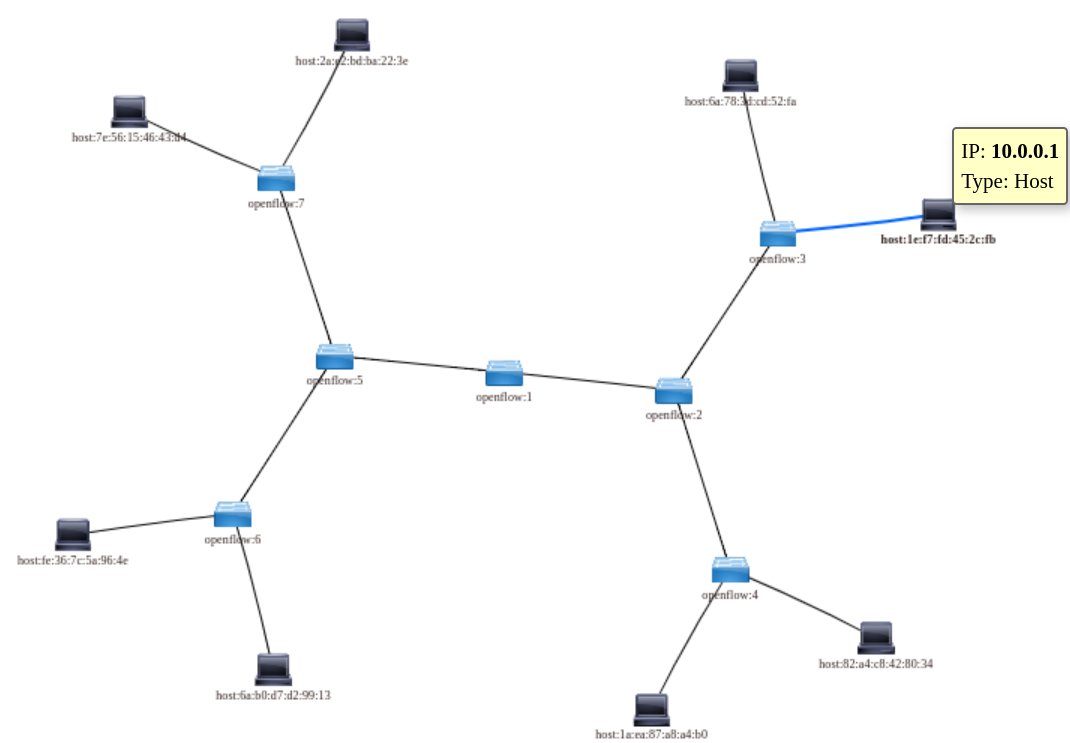
\includegraphics[scale=0.4]{figures/ch5/topo-tree}
	\caption{Tree SDN topology emulated by mininet, and controlled by OpenDayLight Beryllium}
	\label{fig:topo-tree}
\end{figure}

\begin{figure}[!ht]
	\centering
	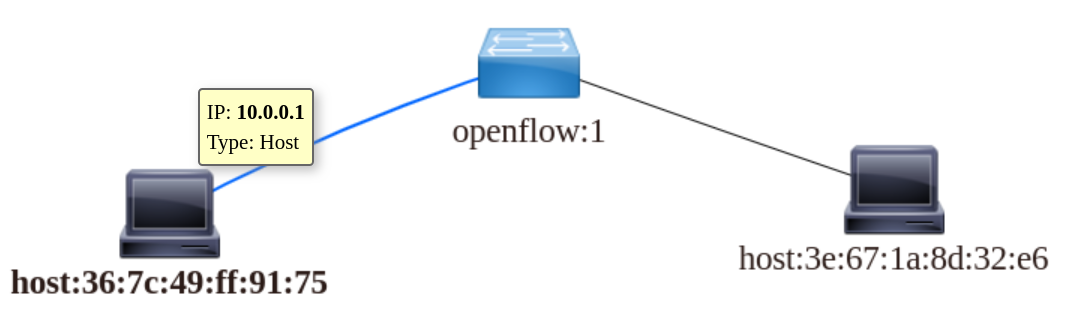
\includegraphics[scale=0.4]{figures/ch5/topo-simple}
	\caption{Single hop SDN topology emulated by mininet, and controlled by OpenDayLight Beryllium}
	\label{fig:topo-simple}
\end{figure}

All Python scripts used to create the scenarios, the Shell Scripts used to automate the tests and capture the traffic, and the Octave scripts to perform all the calculations are available on Github\footnote{\textcolor{red}{github-link}}. To start running the tests, following the tutorial on Github, you should not take more than 10 minutes.

We will perform this testes using SIMITAR \textit{alpha} version, operation as a client on host \textit{h1}, and as a server on all other hosts. As traffic generator engine, we will use D-ITG and Iperf. The operation as a packet injector using Libtins is still unther implementation.

\section{Scalling Evaluation}


To evaluate the Scalling profile of the traccic generator, we are usig the same validation used for Swing\cite{swing-paper}: multiresolution energy analysis.


\section{Packet and Flow Metrics Evaluation}